\section{Ligevægtspunkter og stabilitet}
Stabilitet af et differentialligningssystem er med til at forklare, hvordan systemet opfører sig over tid og er særdeles brugbart i forhold til identificering af ligevægtspunkter. 
\hfill \break

Dette afsnit er baseret på afsnit 7.2 i \citep{EP}. \hfill \break
Et ligevægtspunkt for et differentialligningssystem er et punkt hvor systemet er i ligevægt. Mere præcist defineres det for et autonomt system:
\begin{definition}[Ligevægtspunkt]
Lad 
$$\dot{y} = A\vec{y}$$
være et autonomt lineært differentialligningssystem.
Et ligevægtspunkt for systemet er et punkt $(x_1,x_2 \hdots ,x_n)$ der opfylder ligningen:
$$\dot{y} = A\vec{y}=0$$
\end{definition}

Fasediagrammer er anvendelige i forhold til at illustrere differentialligningssystemer og dermed skabe overblik over opførslen omkring ligevægtspunkter i systemet.\\

Der er givet et system af differentialligninger:

\begin{equation}
    \begin{aligned}
    &\frac{dx}{dt}=F(x,y),\\ 
    &\frac{dy}{dt}=G(x,y)
    \end{aligned}
\end{equation}

Vi kan danne os et overblik over løsningerne til det givne system ved at konstruere et billede, der viser systemets ligevægtpunkter sammen med løsningskurver i $xy$-planet. Dette kaldes et faseportræt, da det illustrere systemets ændringer over tid. \\
\hfill \break
Hvis man ikke med det samme kan gennemskue løsningen til en ODE eller et system, så for at få en idé om hvordan løsningerne kunne se ud kan man konstruere et linjeelement i et $xy$-plan. Her tegner man linjestykker med hældingen:    
$$\frac{dy}{dx}=\frac{y'}{x'}=\frac{G(x,y)}{F(x,y)}$$

\begin{Example}
\hfill \break
\textnormal{Betragt differentialligning systemet:} 

\begin{equation}\label{DLS}
    \begin{aligned}
    &F(x,y)= x'=x-y\\ 
    &G(x,y)=y'=1-x^2
    \end{aligned}
\end{equation}

\textnormal{Med ligevægtspunkterne:} $$(-1,-1) \ \textnormal{og} \ (1,1)$$
\textnormal{}

\textnormal{Ved at kigge på et par tilfældige punkter i $xy$-planet, indsætter deres værdi i (\ref{DLS}) og dermed finde ud af hvad punktets hældning er.} 

\begin{center}
  \begin{tabular}{ | c || c | c | c | c | c |}
    \hline
    x & 0 & 1 & -1 & 0 & $\hdots$ \\ \hline 
    y & 1 & 1 & -1 & -1 & $\hdots$\\ \hline \hline
    $\frac{G(x,y)}{F(x,y)}$ & -1 & 0 & 0 & 1 & $\hdots$\\ \hline
  \end{tabular}
\end{center}

\textnormal{Udfra disse punkter, kan man tegne et linjestykke i hver af punkterne med deres hældning.}

\begin{center}
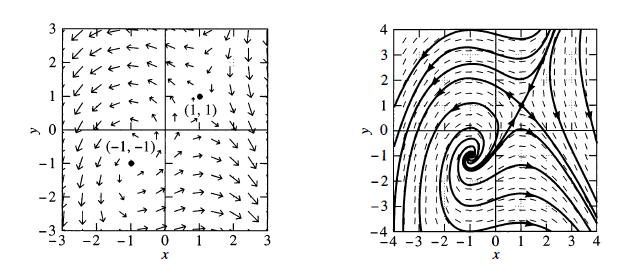
\includegraphics[width=15cm, height=6cm]{slope}
\end{center}
\captionof{figure}{Et linjeelement(tv.) og et faseportæt(th.) til \eqref{DLS}.\citep{EP}} \label{slope}
\hfill \break

\textnormal{På Figur \ref{slope} kan man se hvordan løsningskurverne til i faseportrættet følger linjestykkerne i linjeelementet, og dermed også bevæger sig hhv. hen  imod eller væk fra ligevægtpunkterne.}

\end{Example}

\hfill \break
Vi karakteriserer ligevægtspunkter ud fra løsningskurvernes opførsel omkring dem. Givet et ligevægtspunkt $(x_{1,0},x_{2,0})$ i et autonomt system kaldes dette ligevægtspunkt således for en \textbf{node?} såfremt følgende er gældene for løsningskurverne:
\begin{itemize}
    \item Enten går enhver løsningskurve mod ligevægtspunktet $(x_{1,0},x_{2,0})$ når $t \Rightarrow + \infty$ eller også går enhver løsningskurve væk fra $(x_1,0,x_2,0)$ når $t \Rightarrow + \infty$, og
    \item Enhver løsningskurve er tangent i $(x_{1,0},x_{2,0})$ til en vilkårlig lige linje igennem ligevægtspunktet.  
\end{itemize}
En node kaldes en \textbf{rigtig node} hvis der ikke er to par af modsatliggende løsningskurver, der er tangent til den samme lige linje gennem $(x_{1,0},x_{2,0})$, og kaldes for en \textbf{urigtig node} hvis dette ikke er tilfældet. Dette er illustreret i figur \ref{noder}.
\begin{figure} [H]
    \centering
    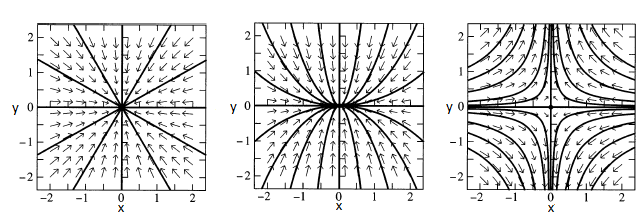
\includegraphics[scale=0.8]{Images/noder.png}
    \caption{En \textbf{Passende/rigtig node} (tv.),en \textbf{ikke-passende/urigtig node} (m) og et saddelpunkt (th.) }
    \label{noder}
\end{figure}

De to ligevægtspunkter til venstre i figur \ref{noder} kaldes også for \textbf{sinks} da alle løsningskurverne går ind mod ligevægtspunktet. Hvis alle løsningskurverne går væk fra ligevægtspunktet, kaldes punktet en \textbf{'kilde'}.

Ligevægtspunktet yderst til højre i figur \ref{noder} kaldes et saddelpunkt. Et saddelpunkt er karakteriseret ved, at mindst en løsningskurve går mod $(x_{1,0},x_{2,0})$, at mindst en løsningskurve bevæger sig væk fra $(x_{1,0},x_{2,0})$ og, at de løsningskurver, der bevæger sig væk fra punktet, er ubegrænsede af $c$.
\\
En mere overordnet metode til beskrivelse af løsningskurvernes opførsel omkring et ligevægtspunkt, er ved brug af begrebet stabilitet.

\begin{definition}[Stabilitet af ligevægtspunkt]
Lad 
$\vec y = A \vec x$
være et autonomt differentialligningssystem, $\vec x_l=(x_1,x_2 \cdots ,x_n)$ et ligevægtspunkt og $\vec x_0=(x_{0,1},x_{0,2} \cdots ,x_{0,n})$ et begyndelsespunkt. Ligevægtspunktet siges at være stabilt såfremt der for hvert $\varepsilon >0$ eksisterer et $\delta >0$ så følgende gælder:
$$|\vec x_0 - \vec x_l|< \delta \Rightarrow |\vec x(t)) - \vec x_l| < \varepsilon $$
\end{definition}
Et ligevægtspunkt kaldes ustabilt, hvis det ikke er stabilt.
Udover at være stabilt kan et ligevægtspunkt også være asymptotisk stabilt, hvilket vil sige, at det udover at være stabilt, også har egenskaben at alle løsningskurver tilstrækkelig tæt på ligevægtspunktet, vil bevæge sig ind mod ligevægtpunktet.

\begin{definition}[Asymptotisk stabilitet af ligevægtspunkt]
Lad 
$\vec y = A \vec x$
være et autonomt differentialligningssystem, $\vec x_l=(x_1,x_2 \cdots ,x_n)$ et ligevægtspunkt og $\vec x_0=(x_{0,1},x_{0,2} \cdots ,x_{0,n})$ et begyndelsespunkt. Ligevægtspunktet siges at være asymptotisk stabilt såfremt der eksisterer et $\delta >0$ så følgende gælder:
$$|\vec x_0 - \vec x_l|< \delta \Rightarrow \lim_{x\to\infty} \vec x(t)= \vec x_l$$
\end{definition}
Det ses således at noderne i figur \ref{noder} også kan beskrives som asymptotisk stabile ligevægtspunkter, mens saddelpunktet er ustabilt. \\
Et såkaldt center(figur \ref{center}), der er defineret ved at alle løsningskurverne former lukkede kurver omkring det, er et eksempel på et stabilt punkt som ikke er asymptotisk stabilt. Mens en spiral (figur \ref{center}) kan være både asymptotisk stabil eller ustabil.

\begin{figure} [H]
    \centering
    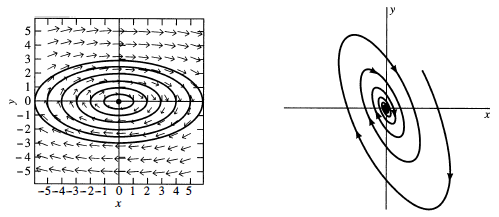
\includegraphics{Images/center.png}
    \caption{Et center (tv.) og en spiral (th.) }
    \label{center}
\end{figure}